\section{Methodology}
\subsection{Basic notions on ABC} Approximate Bayesian Computation or
ABC is a bayesian approach in which the posterior distributions of
the model parameters are determined by replacing the computation of
the likelihood (probability of observed data given the values of the
model parameters) by a measure of similarity between observed and
simulated data. The posterior distributions are estimated from
parameter values providing simulated data that are the most similar
to observed data. Historically, different ways of estimating this
similarity have been proposed, but all have been based on statistics
summarizing information conveyed by the data set. In population
genetics, data most often relate to individuals that have been
genotyped at a given set of loci, these individuals being representative of the
studied populations. The summary statistics are for instance the mean
number of alleles per population or genetic distances between pairs
of populations. It is much easier to measure the
similarity between small sets of summary statistics than between
large sets of multilocus genotype data. When the number of summary
statistics is low, it is possible to select simulated data for which
\emph{all} the summary statistics are close to those of the observed
data \citep{P1999,E2001,EC2003}. However, for more complex scenarios
necessitating a larger number of summary statistics, it becomes
almost impossible to find such simulated data sets. \citet{B2002}
have hence proposed to measure similarity through the Euclidian
distance between observed and simulated summary statistics, after normalization by standard
deviations of simulated statistics. In addition, these authors introduced a
step of local linear regression aimed at favoring simulated data
sets that are closer to the observed one.\\
 In practice, the ABC approach can be summarized in three successive
 steps \citep{Ex2005} : i) generating simulated data sets, ii)
 selecting simulated data sets closest to observed data set and iii)
 estimating posterior distributions of parameters through a local
 linear regression procedure.\\ 
 In addition, this approach provides a way of comparing different
 scenarios that can explain observed data. Two measures of posterior probabilities of scenarios are proposed. The first measure is simply the relative proportion of each scenario in the simulated data sets closest to observed data sets \citep{ME2005,PC2007}. The second measure  is obtained by a logistic regression of each scenario probability on the deviations between simulated and observed summary statistics \citep{FR2007,B2008}. \\
 
 
 In order to simulate data, one has first to define one (or possibly
several) model(s). Each model includes a historical model describing
how the sampled populations  are connected to their common ancestor
and a mutational model describing how allelic states of the studied
genes are changing along their genealogical trees.\\

\subsection{Historical model parameterization}
The evolutionary scenario, which is quantified by the historical
model, can be described as a succession in time of "events" and
"inter event periods". The events considered in the program are a
restricted set of possible events affecting populations evolution.
In the current version of the program, we consider only 4 categories
of events : population divergence, 
discrete change of effective population size, admixture and sampling (the last one has been added
to allow considering samples taken at different times). Between two successive
events affecting a population, we assume that populations evolve
independently (e.g. without migration) and with a fixed effective
size. The usual parameters of the historical model are the times of
occurrence of the various events (counted in generations), the
effective sizes of populations and the admixture rates. When writing
the scenario, events are provided sequentially backward in time.
Although this choice may not be natural at first sight, it is coherent with
coalescence theory on which are based all data simulations in the
program. For that reason, the keywords for a divergence or an
admixture event are \texttt{merge} and \texttt{split}, respectively.
Two other keywords, \texttt{varNe} and \texttt{sample},
correspond to a discrete change in effective population size and a gene
sampling, respectively. Eventually, only for SNPs, we have added the keyword \texttt{refsample} to control the ascertainment bias (see below).\\
A scenario takes the form of a succession of lines (one line per
event), each line starting with the time of the event, then the
nature of the event, and ending with several other data depending on
the nature of the event. Following is the syntax used for each
category of event :
\begin{description}
\item[population sample] : $\langle time \rangle$ \texttt{sample} $\langle pop \rangle$  $[nmales$   $nfemales]$  \\ 
$\langle time \rangle$ is the time (always counted in number of generations) at which the sample was taken and\\
 $\langle pop \rangle$ is the population number from which is taken the sample. It is worth stressing here that \textbf{samples are considered
in the same order as they appear in the data file}.\\
$[nmales$   $nfemales]$ is only used for SNP loci to indicate the number of males (respectively females) from the sample that have been used to detect SNPs. Thes males and females appear in the corresponding sample of the data file.
 
\item[``reference'' sample] : $\langle time \rangle$ \texttt{refsample} $\langle pop \rangle$  $nmales$   $nfemales$  \textbf{ONLY FOR SNP loci}\\ 
$\langle time \rangle$ is the time (always counted in number of generations) at which the ``reference'' sample was taken and\\
 $\langle pop \rangle$ is the population number from which is taken the sample.\\
$nmales$   $nfemales$ indicate the number of males (respectively females) that have been used to detect SNPs in the reference sample. These males and females \textbf{do not appear} in the data file.

\item[population size variation] : $\langle time \rangle$ \texttt{varNe}
 $\langle pop \rangle$ $\langle Ne \rangle$\\
 From time $\langle time \rangle$, looking backward in time,
 population $\langle pop \rangle$ will have an effective size $\langle Ne
 \rangle$.
\item[population divergence] :
$\langle time \rangle$ \texttt{merge} $\langle pop0 \rangle$
$\langle pop1 \rangle$\\
At time $\langle time \rangle$, looking backward in time, population
$\langle pop1 \rangle$ "merges" with population $\langle pop0
\rangle$. Hereafter, only $\langle pop0 \rangle$ "survives".
\item[population admixture] :
$\langle time \rangle$ \texttt{split} $\langle pop0 \rangle$
$\langle pop1 \rangle$ $\langle pop2 \rangle$ $\langle rate \rangle$\\
At time $\langle time \rangle$, looking backward in time, population
$\langle pop0 \rangle$ "splits" between populations $\langle pop1
\rangle$ and $\langle pop2 \rangle$. A gene lineage from population
$\langle pop0 \rangle$ joins population $\langle pop1 \rangle$
(respectively $\langle pop2 \rangle$) with probability $\langle rate
\rangle$ (respectively 1-$\langle rate \rangle$).
\end{description}

A scenario is a succession of lines as described above. However, in
order to cope with special situations (see explanations in Note
 9 below), we added a first line giving the effective sizes of sampled
populations before the first event described, looking backward in time.
Expressions between arrows, other than population numbers, can be
either a numeric value (e.g. 25) or a character string (e.g.
\texttt{t0}). In the latter case, it is considered as a parameter of
the model. So the only possible parameters of the historical model
are times of events, effective population sizes and admixture
rates.\\
The program offers the possibility to add or remove scenarios, by just clicking on the corresponding buttons. The usual shortcuts (CTRL+C, CTRL+V and CTRL+X) can be used to edit the different scenarios. Some or all parameters can be in common among scenarios.\\

\textbf{Notes}
\begin{enumerate}
\item There are two ways of giving a fixed value to effective population sizes, times and admixture rates. Either the fixed value appears as a numeric value in the scenario windows or it  is given as a string value like any parameter. In the latter case, one gives this parameter a fixed value by choosing a Unifom distribution and setting the minimum and maximum to that value in the prior setting (see section 2.4).
\item All expressions must be separated by at least one space.
\item All expressions relative to parameters can include sums or
differences. For instance, it is possible to write :\\
\texttt{t0 merge 2 3}\\
\texttt{t0+t1 merge 1 2}\\
This means that \texttt{t1} is the time elapsed between the two
events. By imposing \texttt{t1>0} (as explained in section
\textbf{prior and posterior distributions}), this implies that the
divergence of populations 1 and 2 is always more ancient than the
divergence of populations 2 and 3. \
However, one cannot mix a parameter and a numeric value (e.g. \texttt{t1+150} will result in an error). This can be done by writing \texttt{t1+t2} and fixing \texttt{t2} by choosing a uniform distribution with lower and upper bounds both equal to 150. 
\item Time is always given in generations. Since we look backward,
time increases towards past.
\item Negative times are allowed (e.g. the example given in section 3), but not recommended.
\item Population numbers must be consecutive natural integers
starting at 1. The number of population can exceed the number of
samples and vice versa : in other words, unsampled populations can be considered in
the scenario on one hand, and the same population can be sampled
more than once on the other hand.
\item Multi-furcating population trees can be considered, by writing
several divergence events occurring at the same time. However, one
has to be careful to the order of the \texttt{merge} events. For
instance, the following piece of scenario will fail :\\
\texttt{100 merge 1 2} \\
\texttt{100 merge 2 3} \\
This is because, after the first line, population 2, which has
merged with population 1, does not "exist" anymore (the surviving population is population 1). So, it cannot
receive lineages of population 3 as it should as a result of the
second line. The correct ways are either to put line 2 before line
1, or to change line 2 to :\\ \texttt{100 merge 1 3}.
\item Since times of events can be parameters, the order of events
can change according to the values taken by the time parameters. In
any case, before simulating a data set, the program sorts out events
by increasing times \footnote{ Sorting events by increasing times can only be done when all time values are known, i.e. when simulating datasets. When checking scenarios, all time values are not yet defined, so that when visualizing a scenario, events are represented in the same order as they appear in the window used to define the scenario.}. If two or more events occur at the same time,
the order is that of the scenario as it is written by the the user.
\item Most scenarios begin with sampling events. We then need to
know the effective size of the populations to perform the simulation
of coalescences until the next event concerning each population. One
way would have been to provide the population size on the same line
of the scenario description. However, in some scenarios with varying
population sizes, it can not be determined what is the effective
size at the sampling time before the set of time parameter values is
generated. For that reason, we decided to provide the effective size
and the sampling description on two distinct lines.
\end{enumerate}

\textbf{Examples} Below are some usual scenarios with increasing complexity. Each scenario is coded on the left side and a graphic representation given by $DIYABC$ is printed on the right side
\begin{enumerate}
\item One population from which several samples have been taken at
various generations : 0, 3 and 10. The only unknown parameter of the scenario\footnote{Of course, there are also one or more parameter(s) for the mutation model.} is the
 effective population size. \\
\begin{center} 
\begin{tabular}{cc}
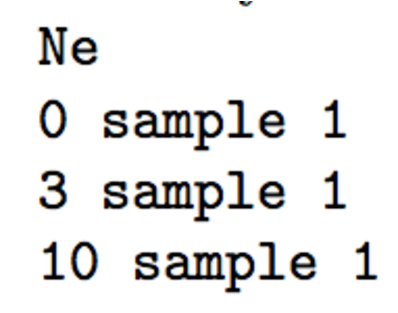
\includegraphics[scale=0.5]{code_scenario_01.pdf} & 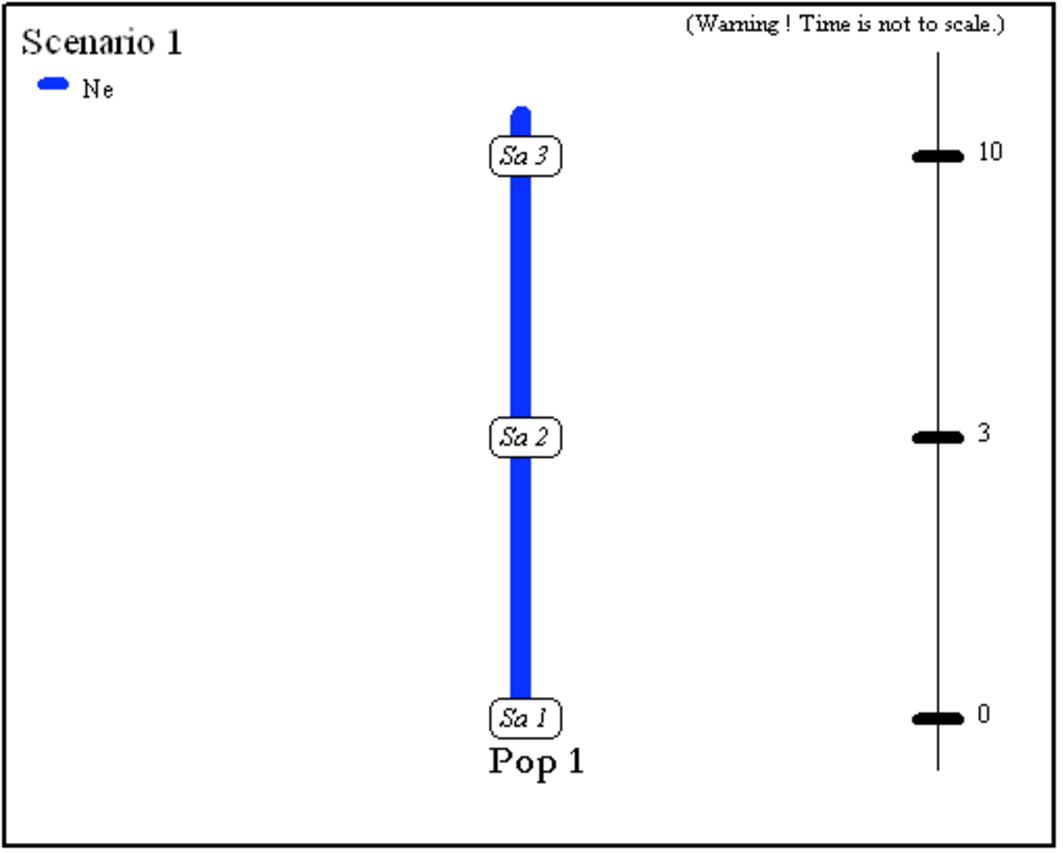
\includegraphics[scale=0.35]{scenario_01.pdf} \\
\end{tabular}
\end{center}

\item Two populations of size \texttt{N1} and \texttt{N2} have diverged \texttt{t} generations
in the past from an ancestral population of size \texttt{N1+N2}.\\
\begin{center} 
\begin{tabular}{cc}
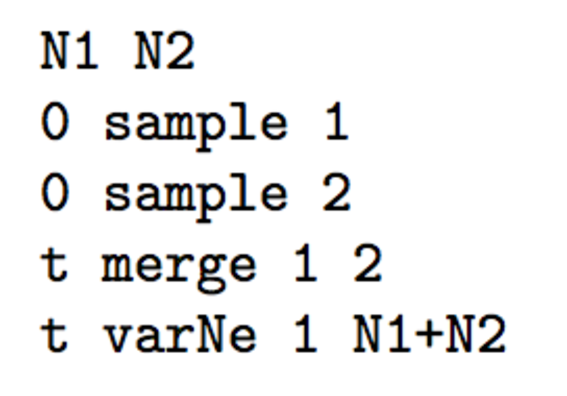
\includegraphics[scale=0.5]{code_scenario_02.pdf} & 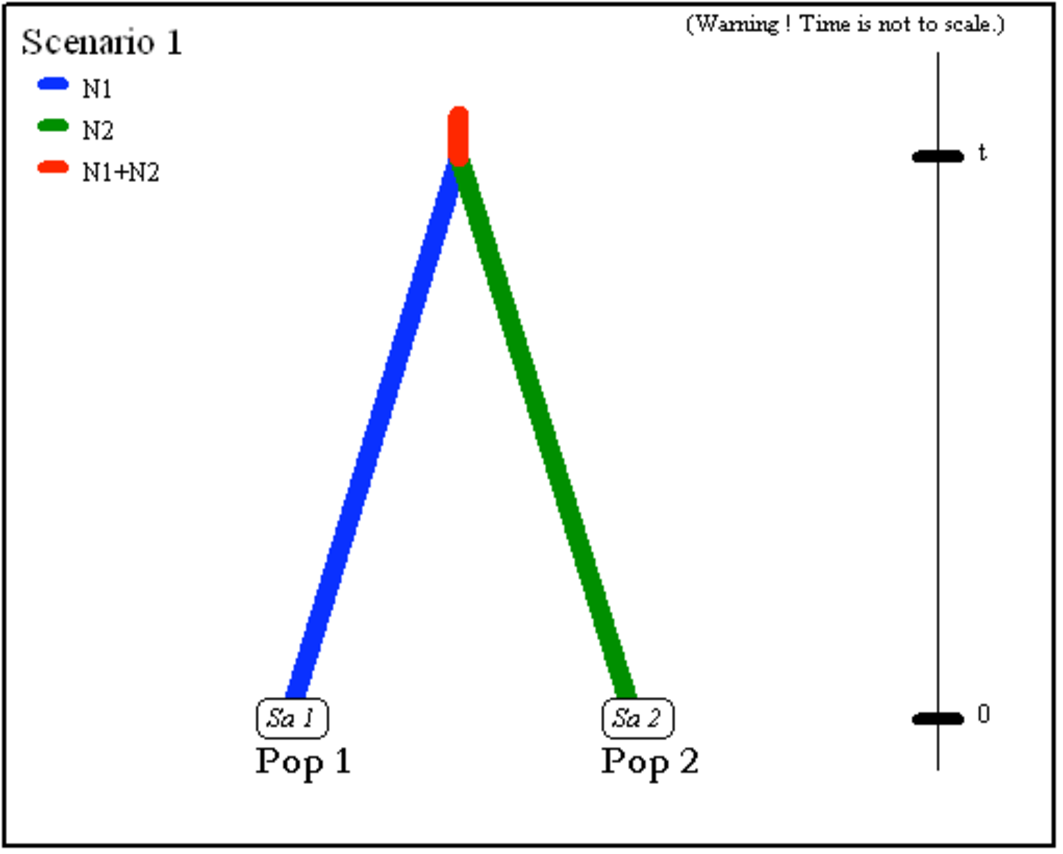
\includegraphics[scale=0.35]{scenario_02.pdf} \\
\end{tabular}
\end{center}


\item Two parental populations (1 and 2) with constant effective populations sizes
\texttt{N1} and \texttt{N2} have diverged at time \texttt{td} from
an ancestral population of size \texttt{NA}. At time \texttt{ta},
there has been an admixture event between the two populations giving
birth to an admixed population (3) with effective size \texttt{N3}
and with an admixture rate \texttt{ra} relative to population 1.\\
\begin{center} 
\begin{tabular}{cc}
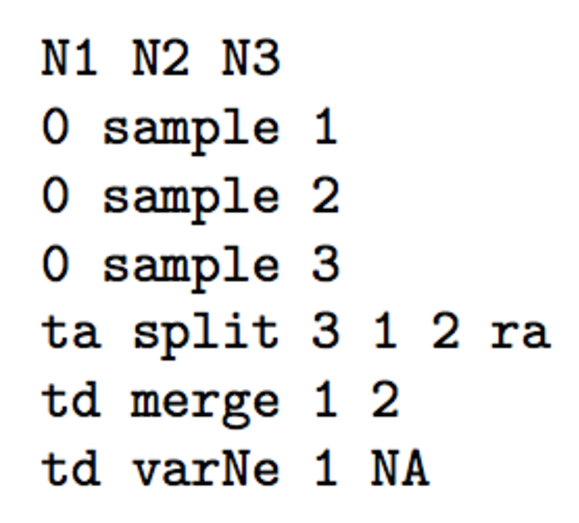
\includegraphics[scale=0.5]{code_scenario_03.pdf} & 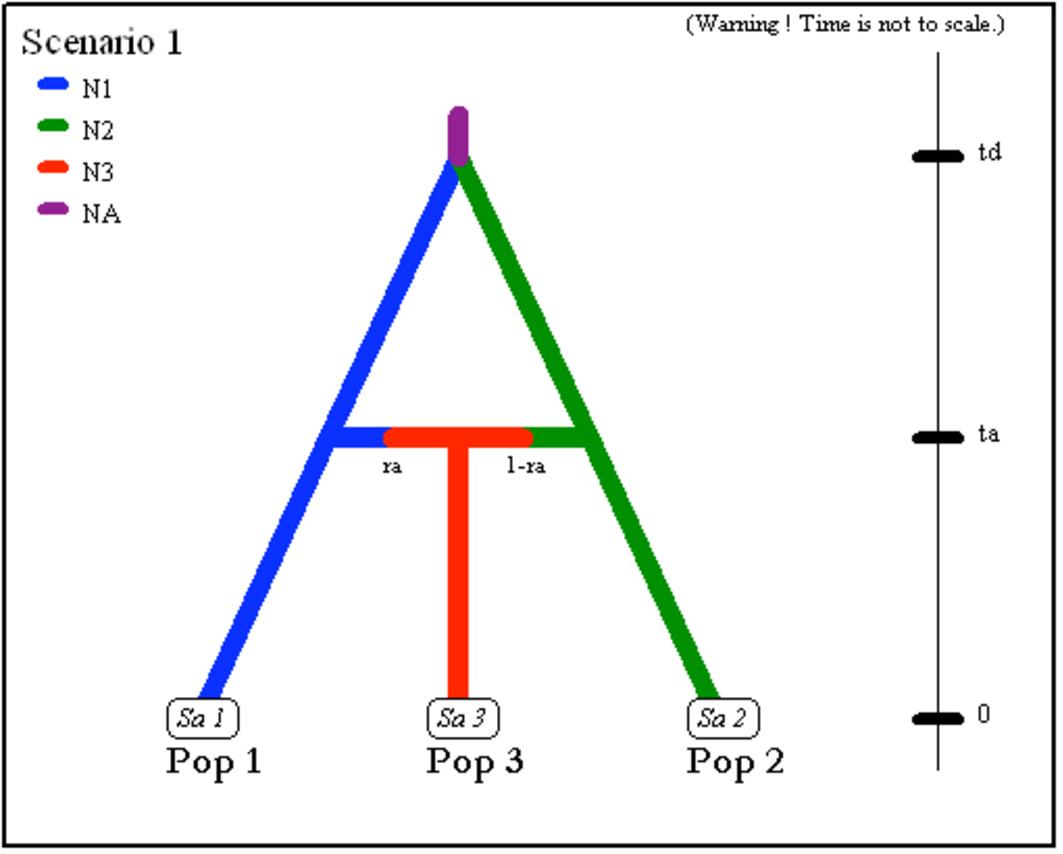
\includegraphics[scale=0.35]{scenario_03.pdf} \\
\end{tabular}
\end{center}

\item The next scenario is slightly more complicated. It includes four population samples and two admixture events.
For simplicity sake, all populations are assumed to have identical effective sizes (\texttt{Ne}).\\
\begin{center} 
\begin{tabular}{cc}
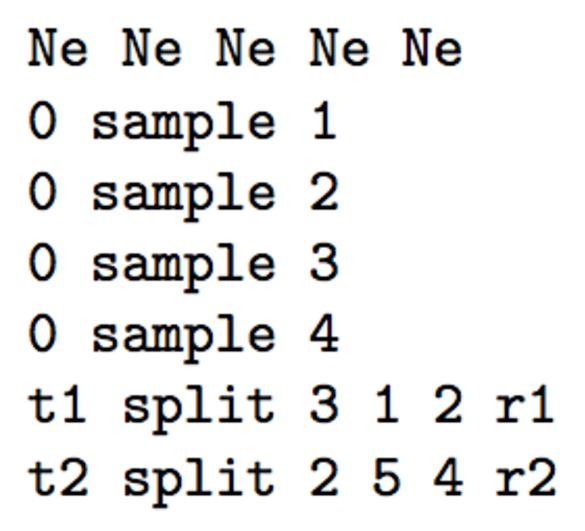
\includegraphics[scale=0.5]{code_scenario_04.pdf} & 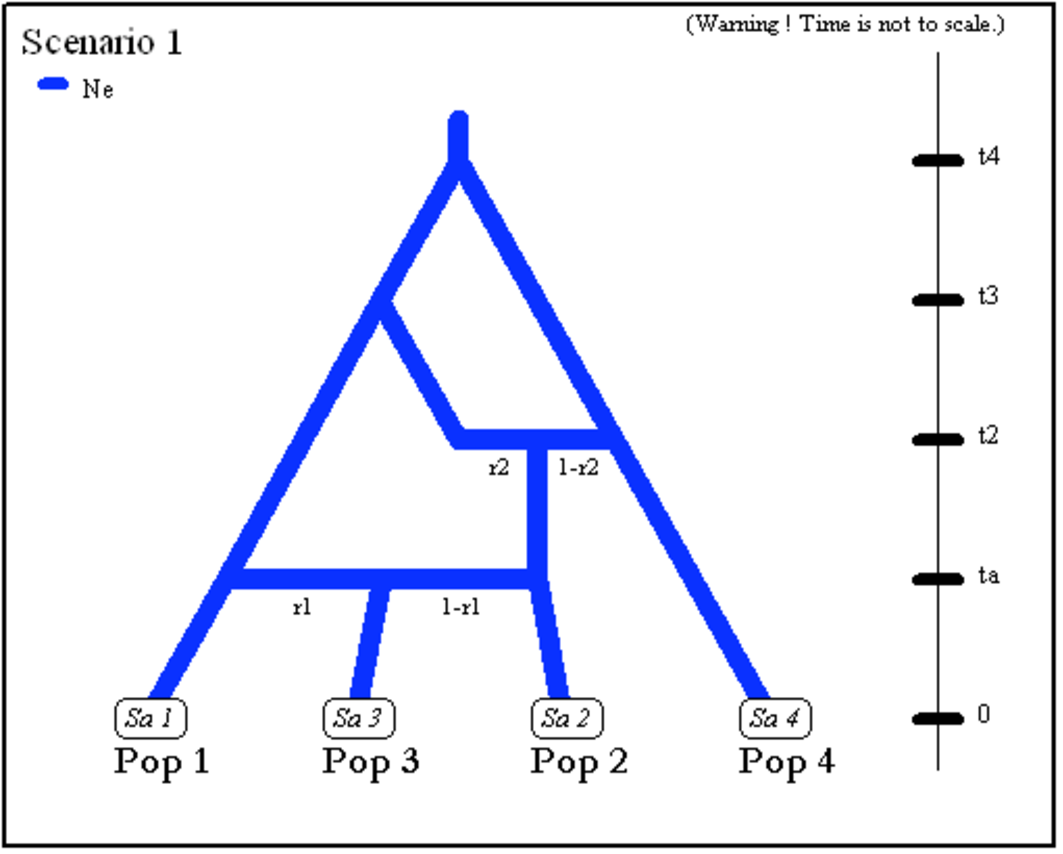
\includegraphics[scale=0.35]{scenario_04.pdf} \\
\end{tabular}
\end{center}



Note that although there are only four samples, the scenario
includes a fifth population. This population which diverged from
population 1 at time \texttt{t3} was a parent in the admixture event
occurring at  time \texttt{t2}. Note also that the first line must include the effective sizes of the \emph{five} populations.\\

\item The following three scenarii correspond to a classic invasion history from an ancestral population (population 1). In scenario 1, population 3 is derived from population 2, itself derived from population 1. In scenario 2, population 2 derived from population 3, itself derived from population 1. In scenario 3, both populations 2 and 3 derived independently from population 1. The same trio of scenarii will be taken later in a fully described example.
Note that when a new population is created from its ancestral population, there is an initial size reduction (noted here \texttt{N2b} for population 2 and  \texttt{N3b} for population 3) since the invasive population generally starts with a few immigrants. 
\end{enumerate}
\medskip \ \ \ \ \ \ \ \  Scenario 1
\begin{center} 
\begin{tabular}{cc}
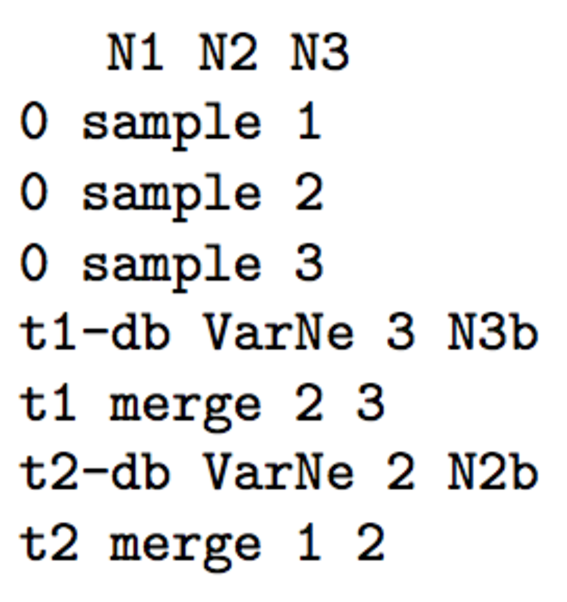
\includegraphics[scale=0.5]{code_scenario_05-1.pdf} & 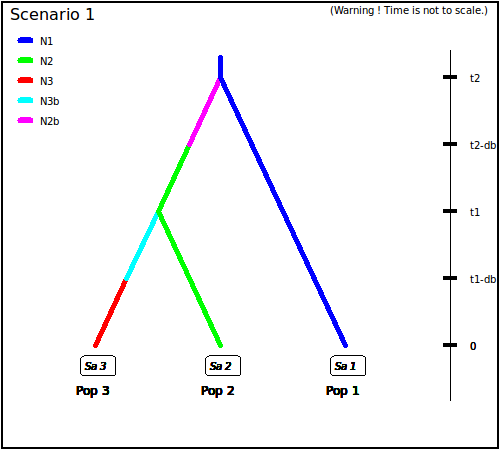
\includegraphics[scale=0.4]{test3pop_scenario_1.png} \\
\end{tabular}
\end{center}

 \ \ \ \ \ \ \ \  Scenario 2
\begin{center} 
\begin{tabular}{cc}
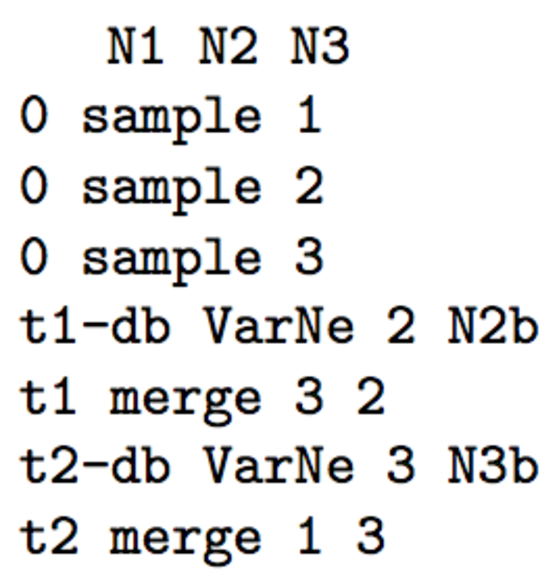
\includegraphics[scale=0.5]{code_scenario_05-2.pdf} & 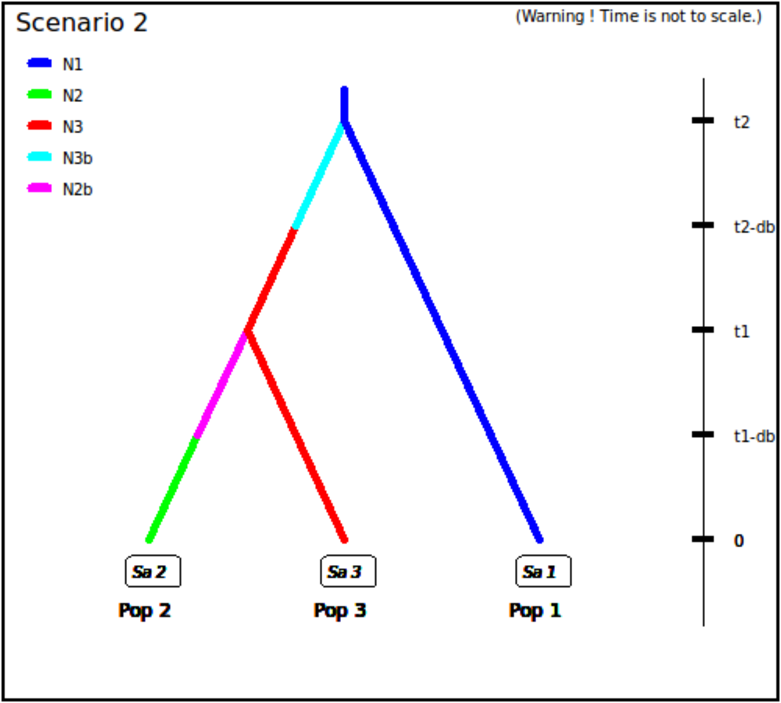
\includegraphics[scale=0.4]{test3pop_scenario_2.pdf} \\
\end{tabular}
\end{center}

\medskip \ \ \ \ \ \ \ \  Scenario 3
\begin{center} 
\begin{tabular}{cc}
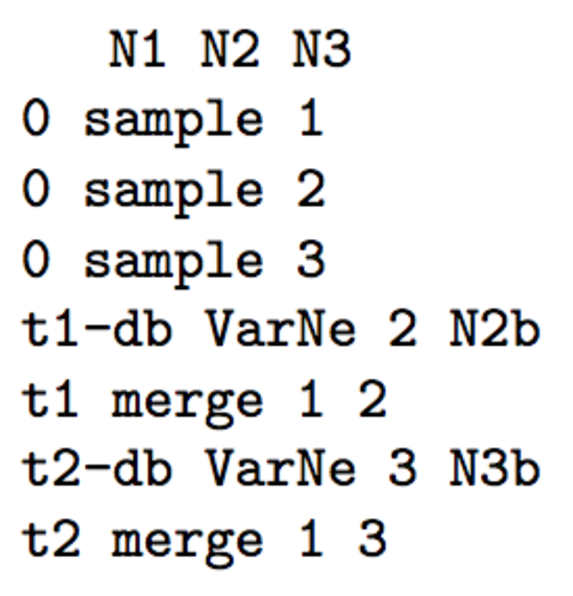
\includegraphics[scale=0.5]{code_scenario_05-3.pdf} & 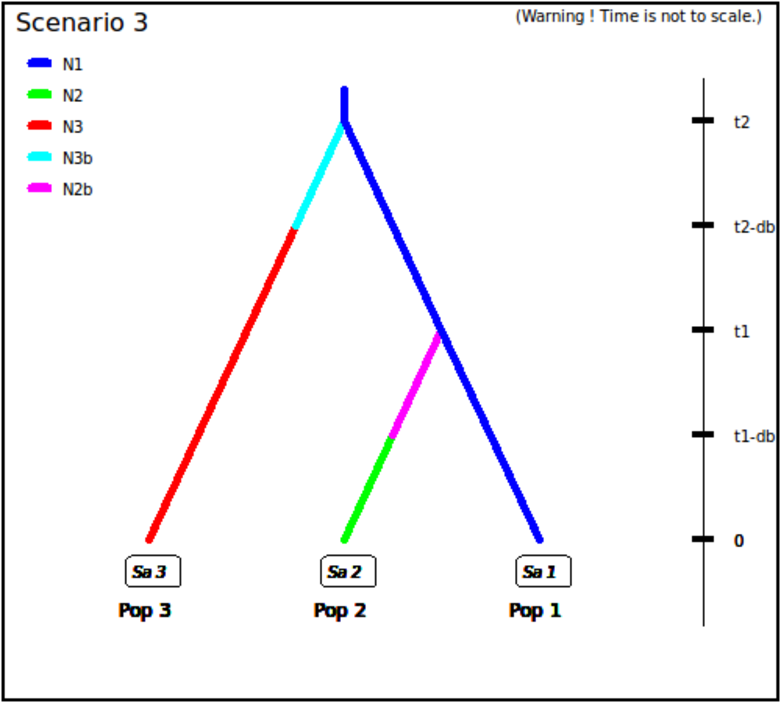
\includegraphics[scale=0.4]{test3pop_scenario_3.pdf} \\
\end{tabular}
\end{center}


\newpage
\subsection{Mutation model parameterization (microsatellite and DNA sequence loci)}
The program can analyse microsatellite data and DNA sequence data altogether as well as separately. In the current version, there  are still two restrictions. First, all loci in an analysis must be genetically independent. Second, for DNA sequence loci, intralocus recombination is not considered.\\

Loci are grouped by the user according to its needs (this an improvement of the current version which imposed all loci of a given category to follow the same mutation model). A different mutation model can be defined for each group. For instance, one group can include all microsatellites with motifs that are 2 bp long and another group those with a 4 bp long motif. Also, with DNA sequence loci, nuclear loci can be grouped together and a mitochondrial locus form a separate group.\\ 
 
The parameterization of the two categories of markers is now described below. 

\subsubsection{Microsatellite loci}
 Although a variety of mutation models have been
proposed for microsatellite loci \citep{W2003}, it is usually
sufficient to consider only the simplest models \citep{C2006}. This
has the non-negligible advantage of reducing the number of parameters, which
can be a real issue when complex scenarios are considered. This is why we chose the Generalized Stepwise Mutation model \citep{E2002}. Under this model, a mutation increases or decreases the length of the microsatellite by a number of repeated motifs  following a geometric
distribution. This model necessitates only two parameters : the mutation rate  (\texttt{$\mu$}) and the parameter of the
geometric distribution (\texttt{$P$}). The same mutation model is imposed to all loci of a given group. However, each locus has its own parameters   (\texttt{$\mu_i$} and \texttt{$P_i$}) and, following a hierarchical scheme, each locus parameter is drawn from a gamma distribution with mean the mean parameter. Note also that :
\begin{enumerate}
\item individual loci parameters (\texttt{$\mu_i$} and \texttt{$P_i$}) are considered as nuisance parameters and hence are never recorded. Only mean parameters are recorded.
\item The variance or shape parameter of the gamma distributions are set by the user and are NOT considered as parameters.
\item The SMM or Stepwise Mutation Model is a special case of the GSM in which the number of repeats involved in a mutation is always one. Such a model can be easily achieved by setting the maximum value of mean P ($\bar{P}$) to 0. In this case, all loci have their $P_i$ set equal to 0 whatever the shape of the gamma distribution.
\item All loci can be given the same value of a parameter by setting the shape of the corresponding gamma distribution to 0 (this is NOT a limiting case of the gamma, but only a way of telling the program). 
\end{enumerate}
Eventually, to give more flexibility to the mutation model, the program offers the possibility to consider mutations that insert or delete a single nucleotide to the microsatellite sequence.  
In the previous version, this option was considered as marginal, and was not treated in the same way as the motif size stepwise mutational process, i.e. there was no associated parameter that could be adjusted to the data. This has been changed in this version :  it is now possible to use a mean parameter (named $ \mu_{(SNI)}$) with a prior to be defined and individual loci having either values identical to the mean parameter or drawn from a Gamma distribution.

\subsubsection{DNA sequence loci}

Note first that this version of the program does not consider insertion-deletion mutations, mainly because there does not seem to be much consensus on this topic. Concerning substitutions, only the simplest models are considered. We chose the Jukes-Cantor (1969) one parameter model, the Kimura (1980) two parameter model, the Hasegawa-Kishino-Yano (1985) and the Tamura-Nei (1993) models. The last two models include the ratios of each nucleotide  as parameters. However, in order to reduce the number of parameters, these ratios have been fixed to the values calculated from the observed data set for each DNA sequence locus. Consequently, this leaves two and three parameters for the Hasegawa-Kishino-Yano (HKY) and Tamura-Nei (TN), respectively.
Also, two adjustments are possible : one can fix the fraction of constant sites (those that cannot mutate) on the one hand and the shape of the Gamma distribution of mutations among sites on the other hand.\\
As for microsatellites, all sequence loci of the same group are given the same mutation model with mean parameter(s) drawn from priors and each locus has its own parameter(s) drawn from a Gamma distribution (same hierarchical scheme). Notes 1, 2 and 4 of previous subsection (2.3.1) apply also for sequence loci.

\subsection{SNPs do not require mutation model parameterization}

SNPs have two characteristics that allow to get rid of mutation models : they are polymorphic and they present only two allelic (ancestral and derived) states. In order to be sure that all analyzed SNP loci have the two characteristics, non polymorphic loci are disgarded right from the beginning of analyses. Consequently, no matter \emph{how} it occurred, we can assume that there occured one and only one mutation in the coalescence tree of sampled genes. We will see below that this  largely simplifies (and speeds up) SNP data simulation. Also, this advantageously reduces the dimension of the parameter space (no mutation parameters which are often considered as nuisance parameters). There is however a potential drawback which is the absence of any calibration generally brought by priors on mutation parameters : only (time/effective size) ratios will be informative.  

\subsection{Prior distributions}
The Bayesian aspect of the ABC approach implies that parameter
estimations are based on prior knowledge about these parameters.
This translates into prior distributions of parameters. The program
offers a choice among usual probability distributions, i.e.
Uniform, Log-Uniform, Normal or Log-Normal for historical parameters and Uniform, Log-Uniform or Gamma
 for mutation parameters. Extremum values and other parameters (e. g. mean and
standard deviation) must be filled in by the
user.  \\
In addition, one can impose some simple conditions on historical
parameters. For instance, there can be two times parameters with
overlapping prior distributions. However, we want that the first
one, say \texttt{t1}, to always be larger than the second one , say
\texttt{t2}. For that, we just need to set \texttt{t1} $>$
\texttt{t2} in the corresponding edit-windows. Such a condition
needs to be between two parameters (not a parameter and a number,
though this can be set up by giving a minimum and a maximum to the
prior distribution) and more precisely between two parameters of the same category (i.e. two effective sizes, two times or two admixture rates). The limit to the number of conditions is
imposed by the logics, not by the program. The only binary
relationships accepted here are $>, <, >= and <=$.

\subsection{Algorithms for data simulation : main features}
Data simulation is based on the Wright-Fisher model. It consists in generating the genealogy of all sampled genes until their most recent common ancestor using coalescence theory.\\ 
This begins by randomly drawing a complete set of
parameters from their own prior distributions and that satisfy all imposed conditions. 
Then, once events have been ordered by increasing times, a sequence
of \emph{actions} is constructed. If there are more than one locus,
the same sequence of actions is used for all successive loci.
Possible \emph{actions} fall into four categories :
\begin{description}
  \item[adding a sample to a population] :\\
Add as many gene lineages to the population as there are genes in
the sample.
  \item[merge two populations] : \\
Move the lineages of the second population into the first
population.
  \item[split between two populations]: \\ Distribute the lineages of the admixed populations between the two
parental population according to the admixture rate.
  \item[coalesce and mutate lineages within a population]: \\
There are two possibilities here, depending on whether the
population is \emph{terminal} or not. We call \emph{terminal} the
population including the most recent common ancestor of the whole
genealogy. In a terminal population, coalescences and mutations stop
when the MRCA is reached whereas in a non terminal population,
coalescence and mutations stop when the upper (most ancient) limit
is reached. In the latter case, coalescences can stop before the
upper limit is
reached because there remains a single lineage, but this single remaining lineage can still mutate.\\
Two different algorithms are implemented : a
generation by generation simulation or a continuous time simulation.
The choice, automatically performed by the program, is based on an empirical criterion which ensures that the (approximate\footnote{The terms \emph{approximate} and \emph{exact} are relative to the basic assumptions of the Wright-Fisher model, not to the biological reality of the process.}) continuous time algorithm is chosen whenever it is faster than the (exact\addtocounter{footnote}{-1}\footnotemark) generation by generation while keeping the relative error on the coalescence rate below 5\% (see  \citet{C2008} for a description of this criterion).\\
 In any case, a coalescent tree is generated over all
 sampled genes.\\
Then the simulation process diverges depending on the type of markers : 
for microsatellite or DNA sequence loci, mutations are distributed over the branches according to a Poisson process whereas for SNP loci, one mutation is applied to a single branch of the coalescent tree, this branch being drawn at random with probability proportional to its length.\\
Eventually, starting from an ancestral allelic state (established as explained below), all allelic states of the
 genealogy are deduced forward in time according to the mutation
 process. For microsatellite loci, the ancestral allelic state is taken at random in the stationary distribution of the mutation model (not considering potential single nucleotide indel mutations). For DNA sequence loci, the procedure is slightly more complicated. First, the total number of mutations over the entire tree is evaluated. Then according to the proportion of constant sites and the gamma distribution of individual site mutation rates, the number and position of mutated sites are generated. Finally, these mutated sites are given 'A', 'T', 'G' or 'C' states according to the selected mutation model. For SNP loci, the ancestral allelic state is arbitrarily set to 0 and it becomes equal to 1 after le the mutation.\\
 Each category of loci has its own coalescence rate deduced from male and female effective population sizes . In order to combine different categories (e.g. autosomal and mitochondrial), we have to take into account the relationships among the corresponding effective population sizes. This can be achieved by linking the different effective population sizes to the effective number of males ( $N_M$ ) and females  ($N_F$) through the sum $N_T=N_F+N_M$ and the ratio $r = N_M/(N_F+N_M)$.  We use the following formulae for the probability of coalescence of two lineages within this population :
 \begin{description}
 \item [autosomal diploid loci :] $p=\frac{1}{8r(1-r)N_T}$
 \item [autosomal haploid loci :] $p=\frac{1}{4r(1-r)N_T}$
 \item [X-linked loci / haplo-diploid loci :] $p=\frac{1+r}{9r(1-r)N_T}$
 \item [Y-linked loci :] $p=\frac{1}{rN_T}$
 \item [Mitochondrial loci :]  $p=\frac{1}{(1-r)N_T}$
 \end{description}
Users have to provide a (total) effective size $N_T$ (on which inferences will be made) and a sex-ratio $r$.
 If no sex ratio is provided, the default value of $r$ is taken as 0.5.  
   

\end{description}
\subsection{Summary statistics}
For each category (microsatellite, DNA sequences or SNP) of loci, the program proposes a series of  summary statistics among those used by population geneticists. These summary statistics are mean values or variances over loci of the same group and 
characterize a single, a pair or a trio of population samples. These are :
\subsubsection{for microsatellite loci}
\begin{description}
\item[Single sample statistics] : 
\begin{enumerate}
  \item mean number of alleles across loci 
  \item mean gene diversity across loci \citep{N1987}
  \item mean allele size variance across loci 
  \item mean M index across loci \citep{GW2001, Ex2005}
 \end{enumerate}
\item[Two sample statistics] :
\begin{enumerate}
  \item $F_{ST}$ between two samples \citep{WC1984}
  \item mean index of classification (two samples) \citep{RM1997,PC2007}
  \item $(\delta\mu)^2$ distance between two samples \citep{GL1995}
  \item mean number of alleles across loci (two samples)
  \item mean gene diversity across loci (two samples)
  \item mean allele size variance across loci (two samples)
  \item shared allele distance between two samples \citep{CJ1993}
  \end{enumerate}
\item[Three sample statistics] :
\begin{enumerate}
  \item Maximum likelihood coefficient of admixture  \citep{CF2004} 
\end{enumerate}
\end{description}

\subsubsection{for DNA sequence loci}

\begin{description}
\item[Single sample statistics] : 
\begin{enumerate}
  \item number of distinct haplotypes 
  \item number of segregating sites
  \item mean pairwise difference
  \item variance of the number of pairwise differences
  \item Tajima's D statistics \citep{TA1989}
  \item Number of private segregating sites (=number of segregating sites if there is only one sample)
  \item Mean of the numbers of the rarest nucleotide at segregating sites\footnote{This statistics can provide information in case of recent demographic variation : a recent expansion increases the number of singletons (nucleotides occuring just once at a segregating site) resulting in a low value of this statistics, whereas a recent decline will produce an opposite result.}
  \item Variance of the numbers of the rarest nucleotide at segregating sites
 \end{enumerate}
\item[Two sample statistics] :
\begin{enumerate}
  \item number of distinct haplotypes in the pooled sample
  \item number of segregating sites in the pooled sample
  \item mean of within sample pairwise differences
  \item mean of between sample pairwise differences
  \item $F_{ST}$ between two samples \citep{H1992}
  \end{enumerate}
\item[Three sample statistics] :
\begin{enumerate}
  \item Maximum likelihood coefficient of admixture  \citep[adapted from][]{CF2004}
\end{enumerate}
\end{description}

\subsubsection{for SNP loci}
\begin{description}
\item[Single sample statistics] : 
\begin{enumerate}
  \item proportion of loci with null gene diverty (= proportion of monomorphic loci) 
  \item mean gene diversity across polymorphic loci \citep{N1987}
  \item variance of gene diversity across polymorphic loci 
  \item mean gene diversity across all loci \citep{GW2001, Ex2005}
 \end{enumerate}
\item[Two sample statistics] :
\begin{enumerate}
  \item proportion of loci with null Nei's distance between the two samples \citep{N1972}
  \item mean across loci of non null Nei's distances between the two samples 
  \item variance across loci of non null Nei's distances between the two samples
  \item mean across loci of Nei's distances between the two samples
  \item proportion of loci with null $F_{ST}$ distance between the two samples \citep{WC1984}
  \item mean across loci of non null $F_{ST}$ distances between the two samples 
  \item variance across loci of non null $F_{ST}$ distances between the two samples
  \item mean across loci of $F_{ST}$ distances between the two samples
  \end{enumerate}
\item[Three sample statistics] :
\begin{enumerate}
  \item Maximum likelihood coefficient of admixture  \citep{CF2004} 
\end{enumerate}
\end{description}

\subsection{Pre-evaluation of scenarios and prior distributions}
This option is proposed to users since version 1.0. The purpose is to check that at least one combination of scenarios and priors can produce simulated data sets that are close enough to the observed data set. This is performed through two kinds of analyses. In the first one, a principal component analysis is performed in the space of summary statistics on at most 100,000 simulated data set and the observed data is added on each plane of the analysis in order to evaluate how the latter is surrounded by simulated data sets. In addition to this global approach, there is a second one in which each summary statistic of the observed data set is ranked against those of the simulated data set. This second analysis helps finding which aspects of the model (including prior) have been mistated. For instance, a grossly overestimated genetic distance (in simulated data sets compared to the observed one) may suggest a mispecification of the prior distribution of the time of divergence of the two involved populations or of the mean mutation rate of the markers. Using this new option before running a full ABC treatment is a convenient way to reveal mispecification of models (scenarios) and/or prior distributions of parameters \citep[see][for an illustration]{C2010}

\subsection{Estimation of posterior distributions of parameters}
Several steps are necessary to get posterior distributions of
parameters. First, the normalized Euclidian distance between the observed data set and
each simulated data set is computed as the sum of squared
differences of summary statistics weighted by the inverse of their
variance in the entire set of simulated data. For the $i$-th data set,
the distance is :
\begin{equation}\label{eq1}
    d_i=\sqrt{\sum_{j=1}^{nstat}\frac{(s_{ij}-s_j^{obs})^2}{V_j}}
\end{equation}
in which $s_{ij}$ is the $j$-th summary statistics from the $i$-th
data set, $s_j^{obs}$ is the $j$-th summary statistics from the
\emph{obs}erved data set and $V_j$ is the variance of the the $j$-th
summary statistics across all simulated data sets.
 Only the closest data sets are selected for further
treatments. The latter includes a local linear regression step aimed
at improving the posterior distributions of the parameters \citep{B2002}. Basically, a
multiple linear regression is performed in which summary statistics
are the independent variables and parameters the dependent
variables. But this regression is also \emph{local} in the sense
that more weight in the regression is given to data sets that are
closest to the observed data set. This is performed by using a
kernel function (the Epanechnikov kernel following \citet{B2002} :
\begin{equation}
\operatorname{K_{\delta}}(d) = \left\{
\begin{array}{ll}
(1.5/\delta)(1-(d/\delta)^2), & t \leq \delta \\
0, & t > \delta \\
\end{array}\right.
\end{equation}
Eventually, parameters are adjusted through this process as :
\begin{equation}\label{eq2}
    \phi_{ik}^*=\phi_{ik}-(\textbf{s}_i-\textbf{s}^{obs})\bm{\beta}_k
\end{equation}
in which $\phi_{ik}$ is the $k$-th parameter of the $i$-th selected
data set, $\phi_{ik}^*$ is the adjusted corresponding parameter,
$\textbf{s}_i$ is the row vector of summary statistics of the $i$-th
selected data set, $\textbf{s}^{obs}$ is the row vector of summary
statistics of the observed data set and $\bm{\beta}_k$ is the
transposed $k$-th row vector of the regression coefficient
matrix.\par The adjusted $\phi_{ik}^*$ of the selected data sets are
an approximate sample of the posterior distribution of parameters \citep{B2002}.

\subsection{Model checking}
\emph{Checking the model is crucial to statistical analysis}  \citep[p161 in][]{GCSR1995}. Model checking (i.e. the assessment of the �goodness-of-fit� of a model � parameter posterior combination) is a facet of ABC analysis that has been so far neglected (but see Ingvarsson,  2008). Following Gelman et al. (1995; pp 159-163), we already implemented this option in $DIYABCv1.0$,  to measure the discrepancy between a model � parameter posterior combination and a �real� data set by considering various sets of test quantities. These test quantities can be chosen among the large set of ABC summary statistics proposed in the program. This option is based on the same kinds of analysis as section 2.7. The main difference is the set of simulated data. Whereas in section 2.7, prior distributions of parameters have been used to simulate data sets, here we use posterior distributions of the same parameters, hence simulating data from the \emph{posterior predictive distribution}. \\
The first analysis is a principal component analysis in the space of summary statistics using data sets simulated with the \textbf{prior} distributions of parameters (exactly as in section 2.7) and the observed data as well as \textbf{data sets from the posterior predictive distribution} are represented on each plane of the PCA. If the model fits well the data, one should see on each PCA plane a wide cloud of data sets simulated from the prior, with the observed data set in the middle of a small cluster of datasets from the posterior predictive distribution.\\
In the second analysis, each summary statistics of the observed data set is ranked against the distribution of the corresponding summary statistics from the posterior predictive distribution. Summary statistics play here the role of \emph{test statistics} \citep[p169 in][]{GCSR1995}.\\
 Since summary statistics are generally not sufficient, it is advised to use different sets of summary statistics to compute the posterior distribution of parameters on one hand and to check the model on the other hand \citep[see][]{C2010}. This has been implemented in $DIYABC$. 

\subsection{Measures of performances}
As stressed in previous studies \citep[e.g.][]{Ex2005}, the ABC appproach provides an efficient way of assessing its own performances for estimating posterior distributions of parameters. The reference table, the building of which represents generally 95 to 99\% of the computing time, can be reused with pseudo-observed (test) data sets which in fact have been obtained through simulation with known values of parameters. It is then rather quick and easy to evaluate the performance of the method for parameter estimation by computing statistics such as estimation biases or mean square errors.\\
These measures of performance have been fully integrated into $DIYABC$. The performance measures computed by $DIYABC$ are :
\begin{description}
\item[the average relative bias] : the difference between the point estimate ($e$) and the true value ($v$)divided by the true value, 
 $\frac{1}{n}\sum_{i=1}^n \frac{e_i - v_i}{v_i}$, averaged over the $n$ test data sets,\\
  \item[the square Root of the Relative Mean Square Error (RRMSE)]: the square root of the average square difference between the point estimate and the true value, divided by the true value,
 $\sqrt{\frac{1}{n}\sum_{i=1}^n(\frac{e_i-v_i}{v_i})^2}$\\
 \item[the square Root of the Relative Mean Integrated Square Error (RRMISE)] : the square root of the average (over test data sets) of the integrated square error (measured on each test data set) divided by the true value,
 $\sqrt{\frac{1}{n}\sum_{i=1}^n(\frac{\sum_{j=1}^{m_i} (x_{ij}-v_i)^2}{m_iv_i^2})}$,
  $x_{ij}$ and $m_i$ being the sampled values and the sample size of the posterior distribution in the $i$-th test data set, respectively.\\
 \item[the Relative Mean Absolute Deviation (RMAD)] : the average (over test data sets) of the mean absolute deviation (measured on each data set), divided by the true value,
 $\frac{1}{n}\sum_{i=1}^n(\frac{\sum_{j=1}^{m_i} \arrowvert x_{ij}-v_i \arrowvert}{m_i \arrowvert v_i\arrowvert}$\\

 \item[the 50\% and 95\% coverages] : the proportion of test data sets for which the 50\% and 95\% credibility intervals respectively include the true value.\\
 \item[the factor 2] :the proportion of test data sets for which the point estimate is at least half and at most twice the true value.
 \item[the Relative Median Bias (RMB)] : the 50\% quantile of the  bias (measured on each data set) divided by the true value. The bias is computed respectively for each point estimate 
 \item[the Relative Median Absolute Deviation (RMedAD)] : the 50\% quantile (over test data sets) of the median (over each data set) of the absolute difference between each value of the posterior distribution sample and the true value divided by the true value.
 \item[the Relative Median of the Absolute Error (RMAE)] :  the 50\% quantile (over test data sets) of the absolute value of the difference between the point estimate (in each data set) and the true value divided by the true value.
\end{description} 
~\
$DIYABC$ considers the following three point estimates : mean, median and mode of the  $\phi_{ik}^*$  (sample of the posterior distribution of each parameter), as defined in subsection 1.7.
~\\
 Concerning the true value ($v$) appearing in the above formulae, DIYABC offers two possibilities :
 \begin{enumerate}
 \item All values $v$ are fixed by the user. If any one of these values is outside the limits given to the prior for the corresponding parameter, a warning message is issued but the analysis can proceed if needed.
 \item All values $v$ are drawn from distributions. These distributions can be different from those of priors. They may even not be overlapping (no warning message is issued whatever the user's choice). 
 \end{enumerate}
 If you want to fix some parameter values and draw the other from distributions, choose the second option and give the same desired values as minimum and maximum for those fixed parameter values.

\subsection{Comparison of scenarios}
The ABC approach can also be used to compare possible scenarios for the same data file through the computation of the posterior probabilities of each scenario and this option is naturally implemented in DIYABC.\\

\subsubsection{Reference table} 
First, the reference table can include as many scenarios as desired. By default, the prior probability of each scenario is uniform, that is each scenario will have approximately the same number of simulated data sets. But, if for any reason, one wants a different prior probability for each scenario, there is the possibility to do so.\\

Scenarios are drawn according to their own prior probability and then only parameters that are defined for the drawn scenario are generated from their respective prior distribution. Scenarios may or may not share parameters.\\
When conditions apply to some parameters (see subsection 2.4), the program provides the possibility of choosing between two options :
\begin{enumerate}
\item parameter sets are drawn in their respective prior distributions until all conditions are fulfilled.
\item a single parameter set is drawn and only if all condition are fulfilled, the simulation is performed and the data set is recorded in the reference table.
\end{enumerate}
When there is only one scenario, both options are equivalent, although in the latter option, there might be less simulated data sets that are recorded than one asked. When there is more than one scenario, the second option can be viewed as a way to set prior probabilities on scenario that result from imposed conditions on parameters (see \citet{ME2005} for an example).  

\subsubsection{Posterior probability of scenarios}
The program $DIYABC$ provides two estimates of the posterior probability of each scenario :
\begin{description} 
\item[a \emph{direct}  estimate :] This is simply the number of times that a given scenario is found in the first $n_{\delta}$ simulated data sets once the latter, produced under several scenarios, have been sorted by ascending distances to the observed data set.\\
\item[a logistic regression estimate :] Following M.A. Beaumont's suggestion \citep{FR2007,B2008}, a polychotomic weighted logistic regression is performed on the first  $n_{\delta}$ data sets with the proportion of the scenario as the dependent variable and the differences between observed and simulated data set summary statistics as the independent variables. The intercept of the regression (corresponding to an identity between simulated and observed summary statistics) is taken as the point estimate. In addition, 95\% confidence intervals are computed \citep{C2008}. 
\end{description} 

Since both estimates are dependent upon the chosen threshold ($\delta$), the program provides a range of 100 estimates for the direct approach (for each one 100-th of $n_{\delta}$ between 0 and $n_{\delta}$) and up to 10 estimates for the logistic regression estimates (e.g. one estimate for $kn_{\delta}/10$ with $k \in[1,2,...10]$ when the number of analyses is set to 10). These estimates are represented in two graphs, one for each kind of estimate. These two graphs can be printed and/or saved (in \emph{svg}, \emph{jpg}, \emph{png} or \emph{pdf} format). Values can also be output as a text file.\

\subsubsection{Confidence in scenario choice}
The program DIYABC offers a last option that allows one to evaluate the confidence in a scenario choice. Suppose that we compare 3 scenarios for a given data set and that e.g. scenario 2 had maximum posterior probability. By using this option, we can estimate type I and type II errors when choosing scenario 2 as the true scenario. To do so, we simulate a given number of data sets according to scenario 1, 2 and 3. Then we count the proportion of times that scenario 2 has not the highest posterior probability among the three competing scenarios when it is the true scenario (type I error, estimated from test data sets simulated under scenario 2) or the proportion of times that scenario 2 has highest posterior probability when it $not$ the true scenario (type II error, estimated from test data sets simulated under scenarios 1 and 3).\\

In $DIYABCv2.0$, a new possibility is offered to the user that may be useful when dealing with many summary statistics and many scenarios. In this particular case, the logistic regression has to deal with large matrices and the amount of needed memory on one hand and the computation time on the other hand can become problematically large. An approximate solution is to replace summary statistics by the components of a factorial discriminant analysis which reduces the number of independent variables to the smallest of number of summary statistics and scenarios. Although the result is only approximate, it can be a useful guide in some specific cases. The gain in time can be large. For instance, the time can be reduced by a 30X factor. \\

As for the bias/precision analysis, parameter values can be fixed to given values or drawn from given distributions (not necessarily the same as those used as priors for the reference table).

\clearpage
